\section{Chain C -- Subscriber, 200-msg Gate and Router}

Subscribes to the same topic, applies a hard cap of 200 processed
messages, computes $N = \mathit{id} \bmod 5218$, retrieves the matching
row from the cached CSV, and dispatches it to one of three
sub-flows (ZCL handler, Link Status handler, or drop).

\begin{figure}[h]
    \centering
    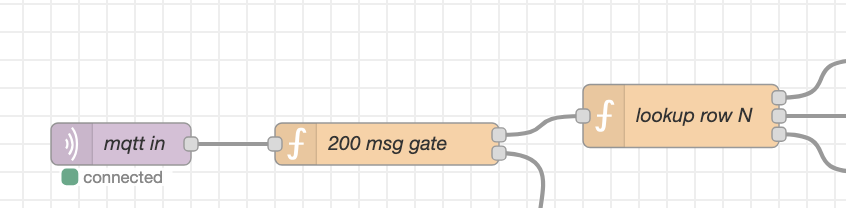
\includegraphics[width=0.95\linewidth]{images/flow_chain_c.png}
    \caption{Chain C -- subscriber, message gate and router.}
\end{figure}

\begin{description}
    \item[MQTT in] subscribes to \texttt{challenge3/id\_generator} with
        \emph{parsed JSON object} output, exposing
        \verb|msg.payload.id| and \verb|msg.payload.timestamp|.
    \item[Function \emph{200-msg gate}] increments a counter on
        \emph{every} arrival; once it reaches 200 a single
        end-of-execution message is emitted on output~2 and all later
        messages are dropped. Ignored messages still consume budget,
        as required.
        \begin{lstlisting}[]
        let count = flow.get('subCount') || 0;
        if (count >= 200) return [null, null];
        
        count++;
        flow.set('subCount', count);
        
        let eof = null;
        if (count === 200) {
            eof = { payload: "end_of_execution" };
            node.warn("Reached 200 messages -- triggering EOF.");
        }
        msg.subCount = count;
        return [msg, eof];
        \end{lstlisting}
    \item[Function \emph{Lookup row N}] computes $N$, fetches
        \verb|global.challengeCsv[N]|, attaches the row, the
        \texttt{SUB\_ID} and the \texttt{Command String} to
        \verb|msg.lookup|, and routes the message to one of three
        outputs by inspecting the Command String for the substrings
        \texttt{ZBEE\_ZCL} or \texttt{Link Status (0x08)}.
        \begin{lstlisting}[]
        const id = msg.payload.id;
        const N = id % 5218;
        const csv = global.get('challengeCsv');
        if (!csv) { node.warn("CSV not loaded yet!"); return null; }
        
        const row = csv[String(N)];
        if (!row) { node.warn(`No row for N=${N}`); return null; }
        
        const cmdStr = row["Command String"] || "";
        msg.lookup = { subId: id, N: N, row: row, cmdStr: cmdStr };
        
        if (cmdStr.includes("ZBEE_ZCL")) { msg.topic = "zcl";  return [msg, null, null]; }
        else if (cmdStr.includes("Link Status (0x08)")) { msg.topic = "linkstatus"; return [null, msg, null]; }
        else { msg.topic = "ignore"; return [null, null, msg]; }
        \end{lstlisting}
\end{description}